\documentclass{article}
\title{Homework5.1}
\author{Blue\&Megan}
\date{20230316}
\usepackage{geometry}
\geometry{a4paper,scale=0.8}
\usepackage{graphicx}
\usepackage{float}
\usepackage{indentfirst}
\usepackage[namelimits]{amsmath} %数学公式
\usepackage{amssymb}             %数学公式
\usepackage{color}
\usepackage{longtable}
\usepackage{listings}
\lstset{
language=Matlab,
numbers=left,
keywordstyle=\color{blue},
numberstyle=\tiny,
breaklines=true,
extendedchars=flase
}
\begin{document}
\maketitle
\section{"Naive" stochastic simulation}
Here we set $n_0=1000,k=2,\Delta t=0.001$. We stimulate it 4 times and get the following result.
\begin{figure}[htbp]
    \centering
    \begin{minipage}{0.45\linewidth}
        \centering
        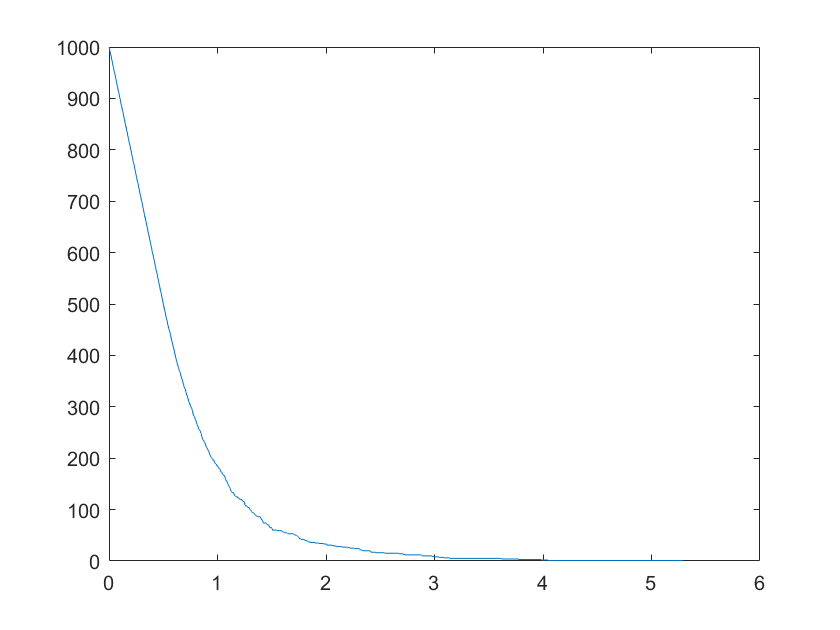
\includegraphics[width=\linewidth]{graph/a1.png}
        \caption{Simulation1}
        \label{a1}
    \end{minipage}
    \hfill
    \begin{minipage}{0.45\linewidth}
        \centering
        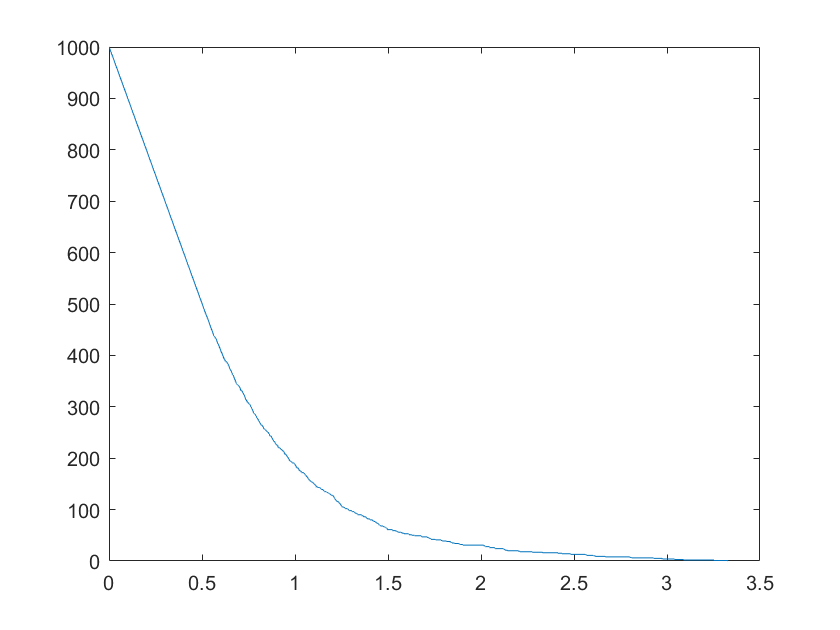
\includegraphics[width=\linewidth]{graph/a2.png}
        \caption{Simulation2}
        \label{a2}
    \end{minipage}
\end{figure}

\begin{figure}[htbp]
    \centering
    \begin{minipage}{0.45\linewidth}
        \centering
        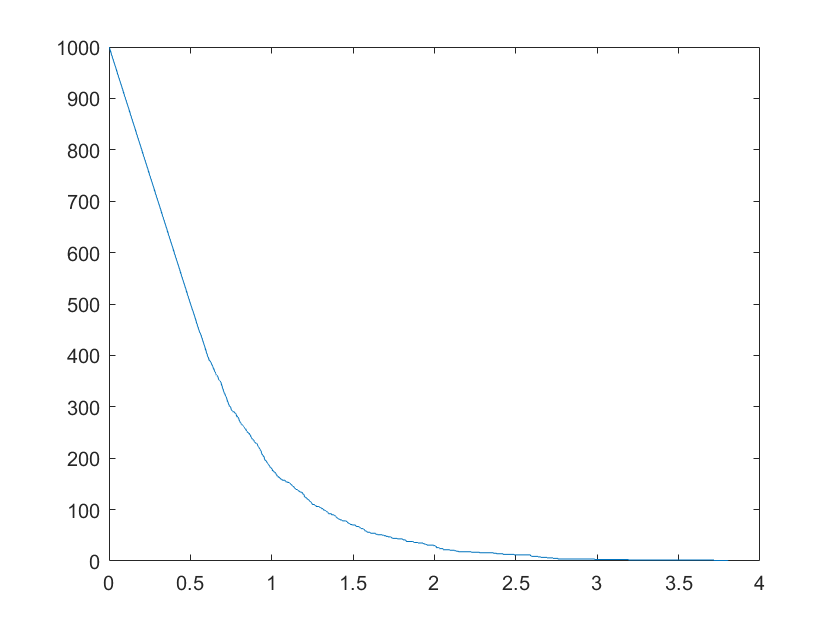
\includegraphics[width=\linewidth]{graph/a3.png}
        \caption{Simulation3} 
        \label{a3}
    \end{minipage}
    \hfill
    \begin{minipage}{0.45\linewidth}
        \centering
        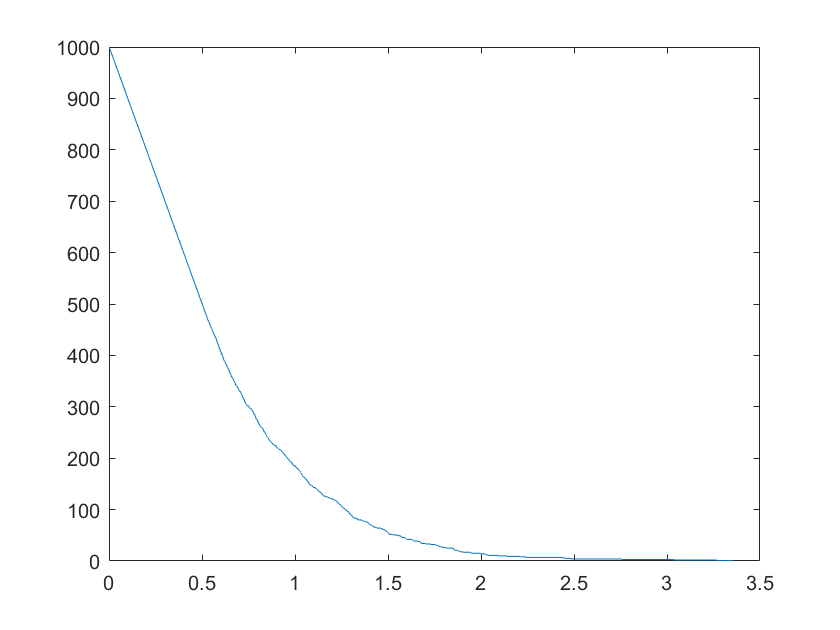
\includegraphics[width=\linewidth]{graph/a4.png}
        \caption{Simulation4}
        \label{a4}
    \end{minipage}
\end{figure}
\clearpage


\section{Gillespie stochastic simulation algorithm}
Here we set $n_0=100,k=2$. We simulation it 10 times and print the deterministic function on the same plot. Then we print the mean.
\begin{figure}[htbp]
    \centering
    \begin{minipage}{0.45\linewidth}
        \centering
        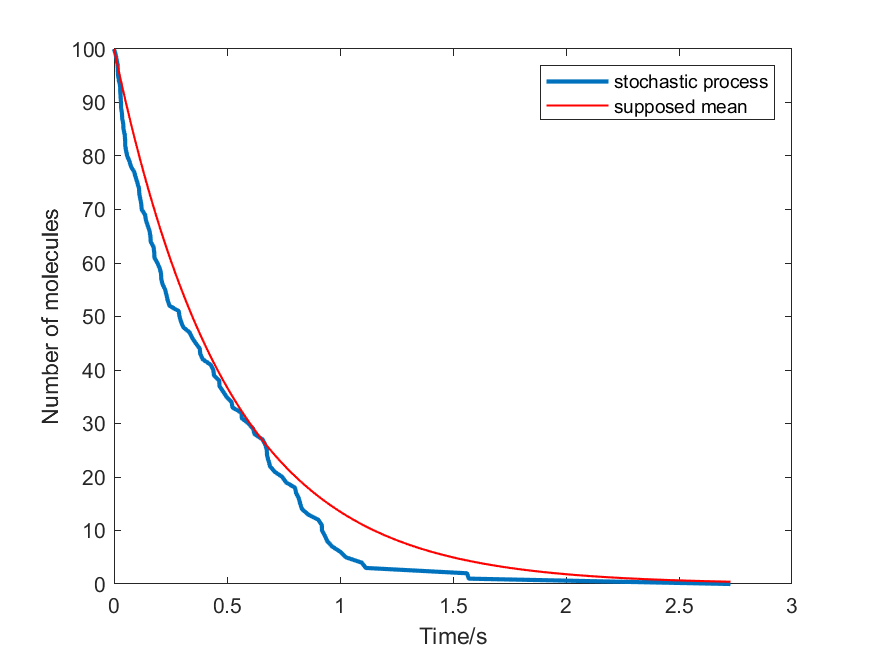
\includegraphics[width=\linewidth]{graph/b1.png}
        \caption{Simulation1}
        \label{b1}
    \end{minipage}
    \hfill
    \begin{minipage}{0.45\linewidth}
        \centering
        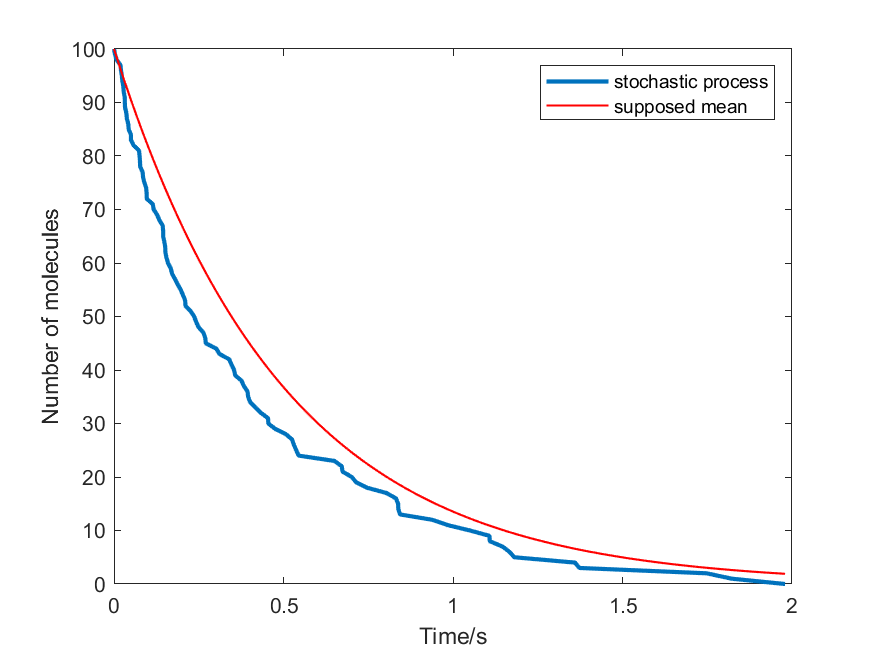
\includegraphics[width=\linewidth]{graph/b2.png}
        \caption{Simulation2}
        \label{b2}
    \end{minipage}
\end{figure}
\begin{figure}[htbp]
    \centering
    \begin{minipage}{0.45\linewidth}
        \centering
        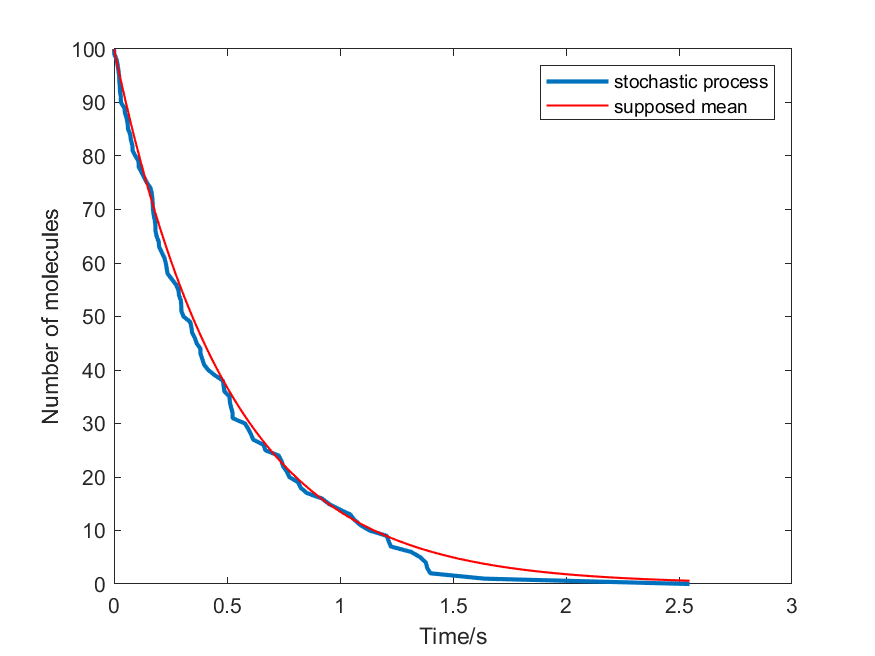
\includegraphics[width=\linewidth]{graph/b3.png}
        \caption{Simulation3}
        \label{b3}
    \end{minipage}
    \hfill
    \begin{minipage}{0.45\linewidth}
        \centering
        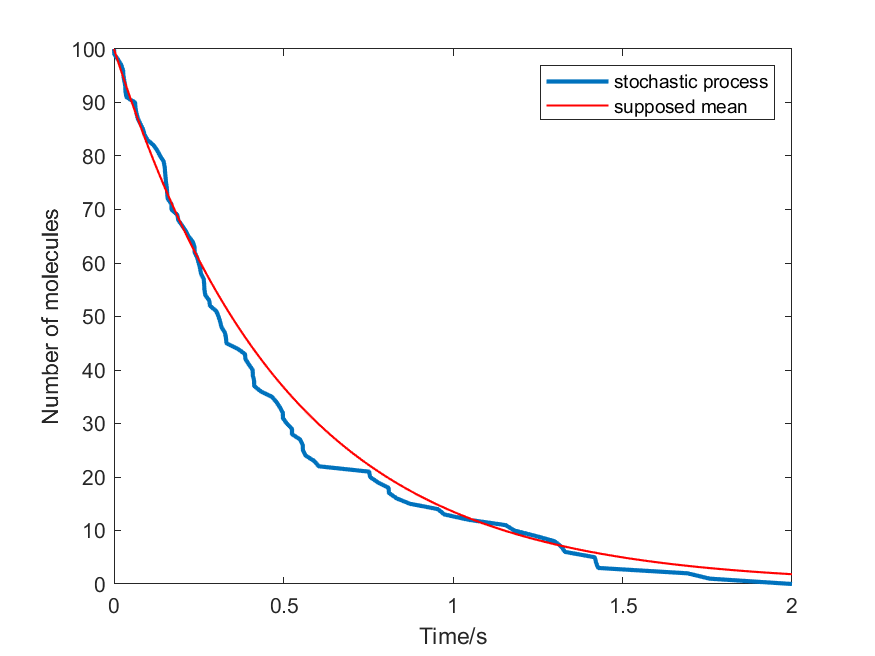
\includegraphics[width=\linewidth]{graph/b4.png}
        \caption{Simulation4}
        \label{b4}
    \end{minipage}
\end{figure}
\begin{figure}[htbp]
    \centering
    \begin{minipage}{0.45\linewidth}
        \centering
        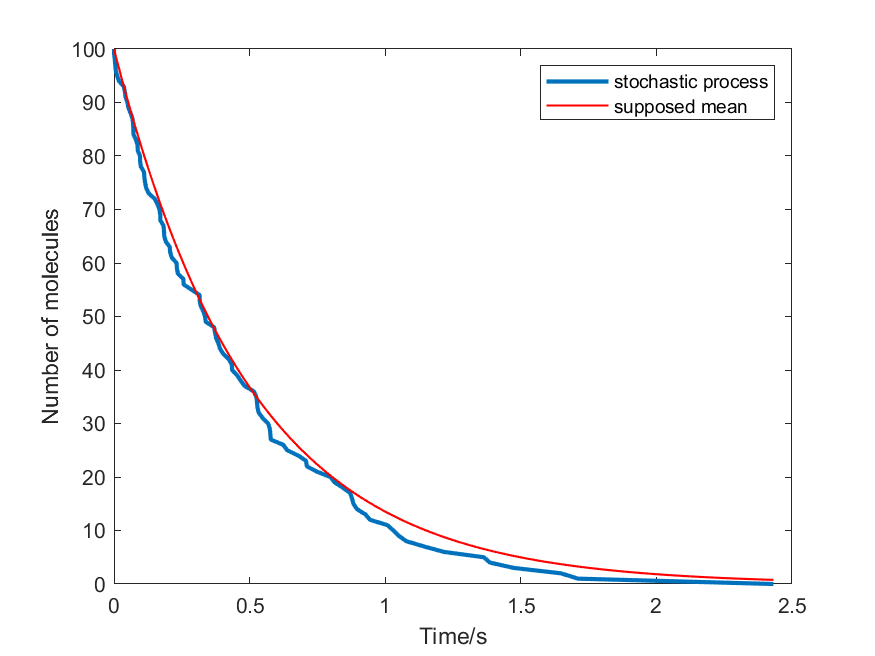
\includegraphics[width=\linewidth]{graph/b5.png}
        \caption{Simulation5}
        \label{b5}
    \end{minipage}
    \hfill
    \begin{minipage}{0.45\linewidth}
        \centering
        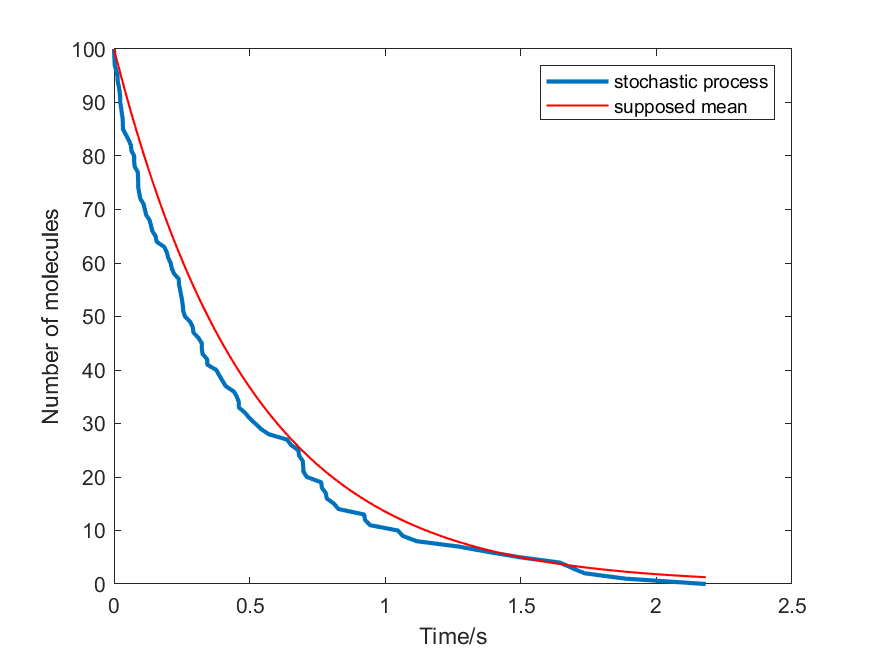
\includegraphics[width=\linewidth]{graph/b6.png}
        \caption{Simulation6}
        \label{b6}
    \end{minipage}
\end{figure}
\begin{figure}[htbp]
    \centering
    \begin{minipage}{0.45\linewidth}
        \centering
        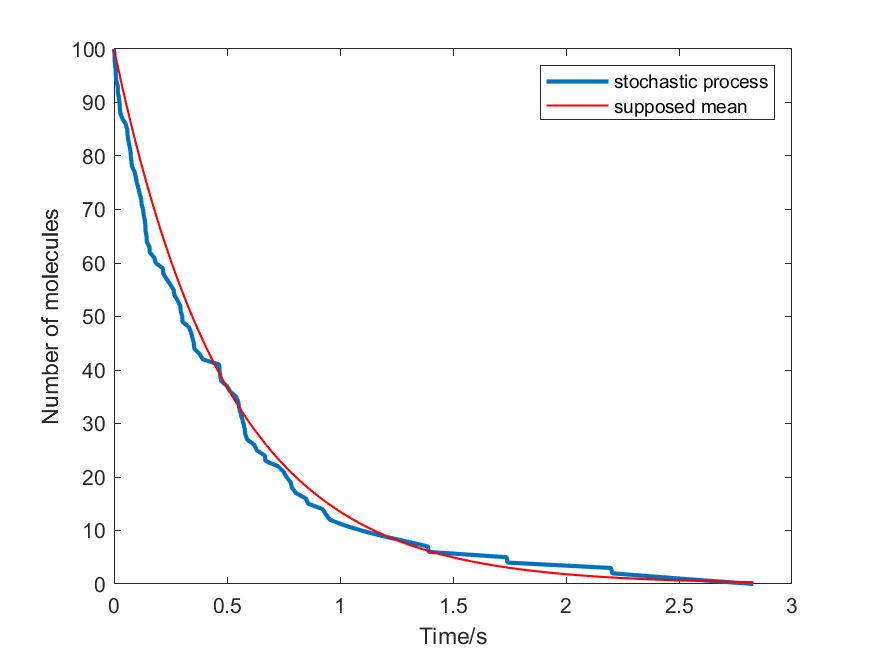
\includegraphics[width=\linewidth]{graph/b7.png}
        \caption{Simulation7}
        \label{b7}
    \end{minipage}
    \hfill
    \begin{minipage}{0.45\linewidth}
        \centering
        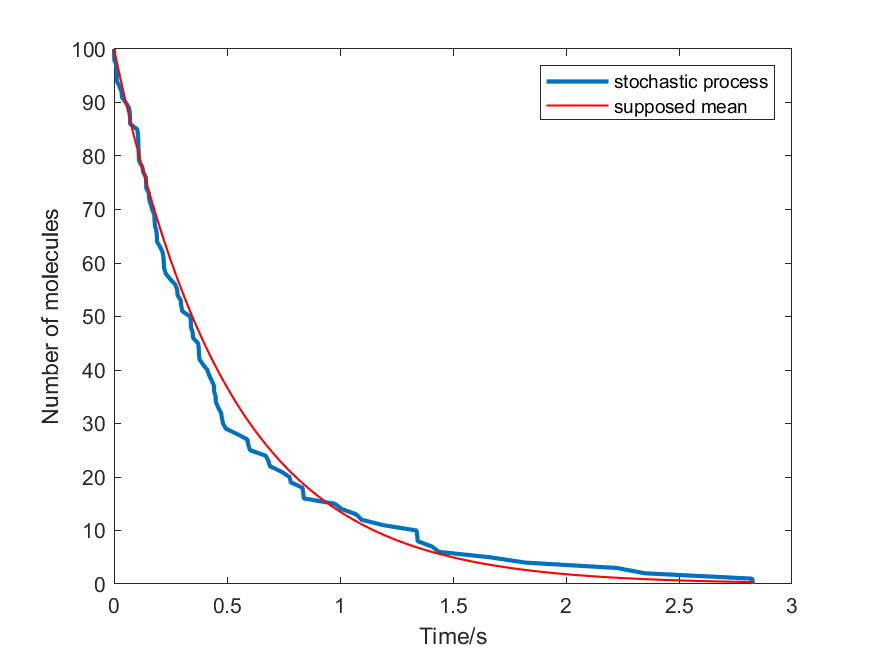
\includegraphics[width=\linewidth]{graph/b8.png}
        \caption{Simulation8}
        \label{b8}
    \end{minipage}
\end{figure}
\begin{figure}[htbp]
    \centering
    \begin{minipage}{0.45\linewidth}
        \centering
        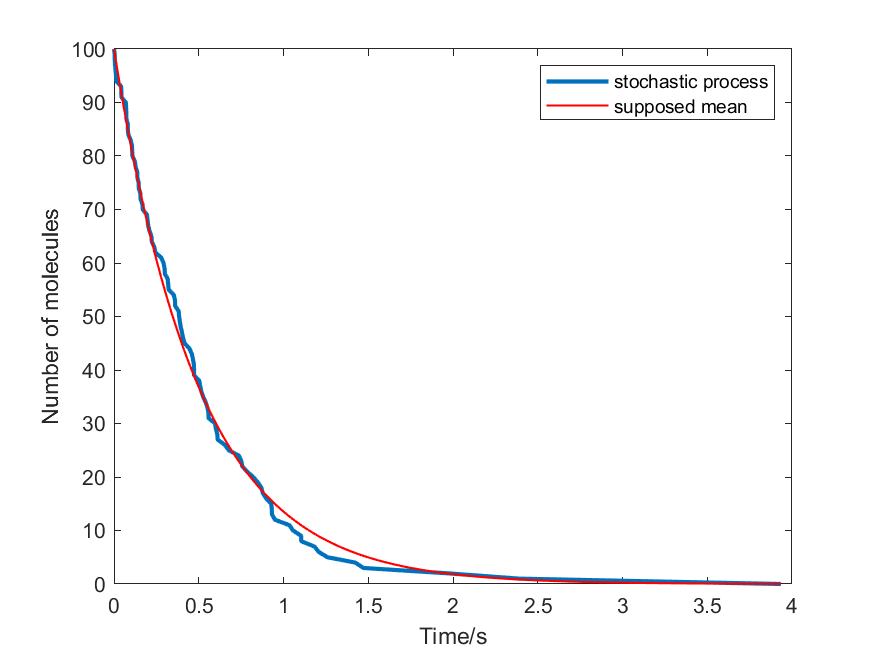
\includegraphics[width=\linewidth]{graph/b9.png}
        \caption{Simulation9}
        \label{b9}
    \end{minipage}
    \hfill
    \begin{minipage}{0.45\linewidth}
        \centering
        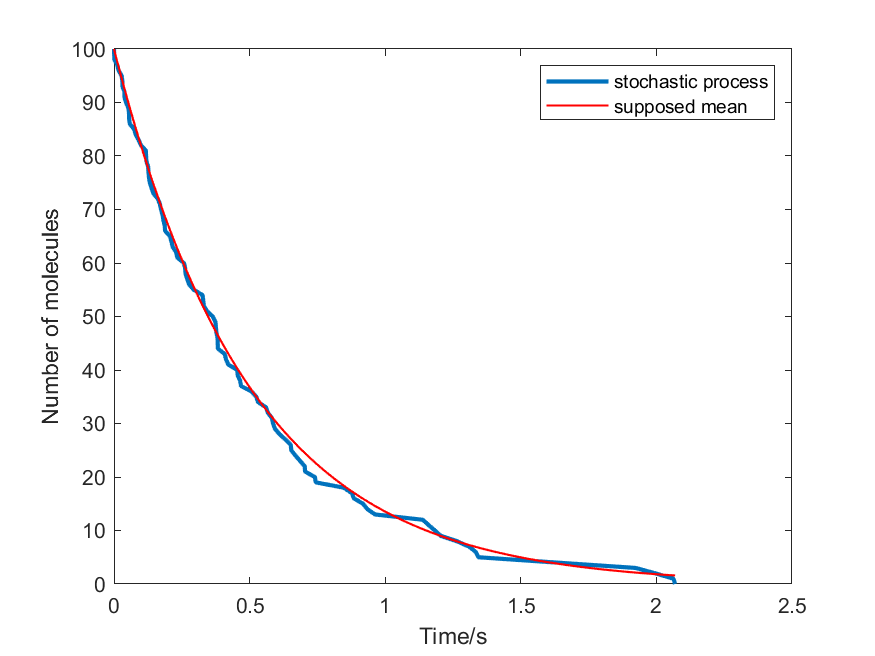
\includegraphics[width=\linewidth]{graph/b10.png}
        \caption{Simulation10}
        \label{b10}
    \end{minipage}
\end{figure}
\begin{figure}[htbp]
\centering
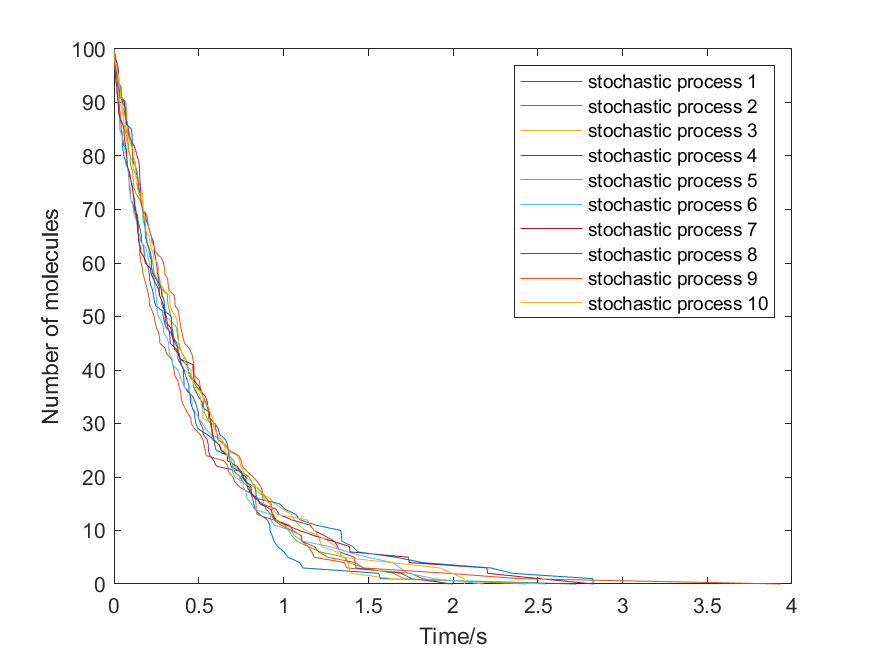
\includegraphics[width=\linewidth]{graph/mean1.png}
\caption{mean}
\end{figure}
\clearpage



\section{Gillespie SSA for 2 reactions}
First, we compute the deterministic function and get:
\begin{equation}
a=\frac{k_2}{k_1}+\frac{N_0-\frac{k2}{k1}}{\exp^{k_1}t}
\end{equation}
Then we set $n_0=100,k_1=2,k_2=4$. We simulation it 10 times and print the deterministic function on the same plot.Then we print the mean.
\begin{figure}[htbp]
    \centering
    \begin{minipage}{0.45\linewidth}
        \centering
        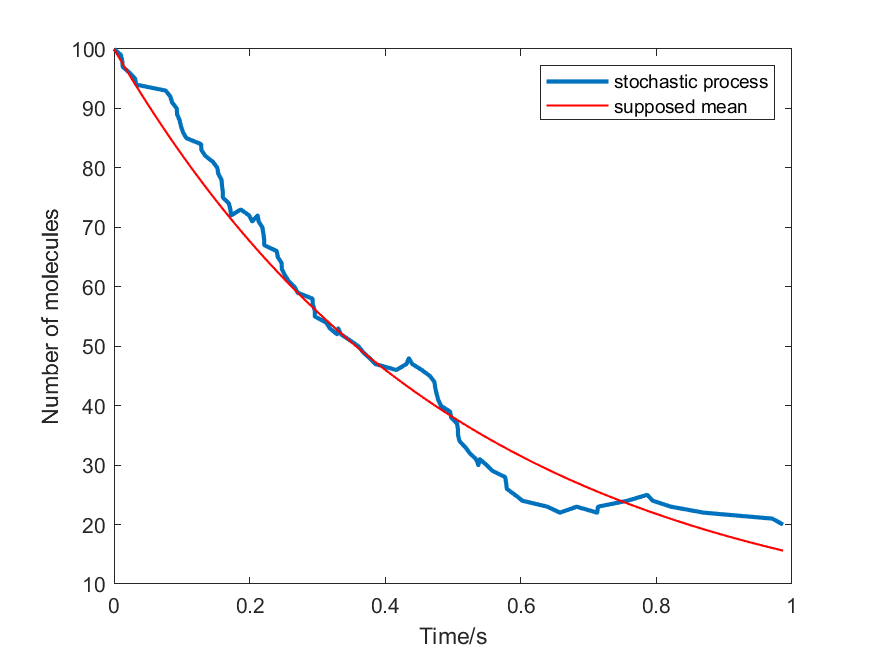
\includegraphics[width=\linewidth]{graph/c1.png}
        \caption{Simulation1}
        \label{c1}
    \end{minipage}
    \hfill
    \begin{minipage}{0.45\linewidth}
        \centering
        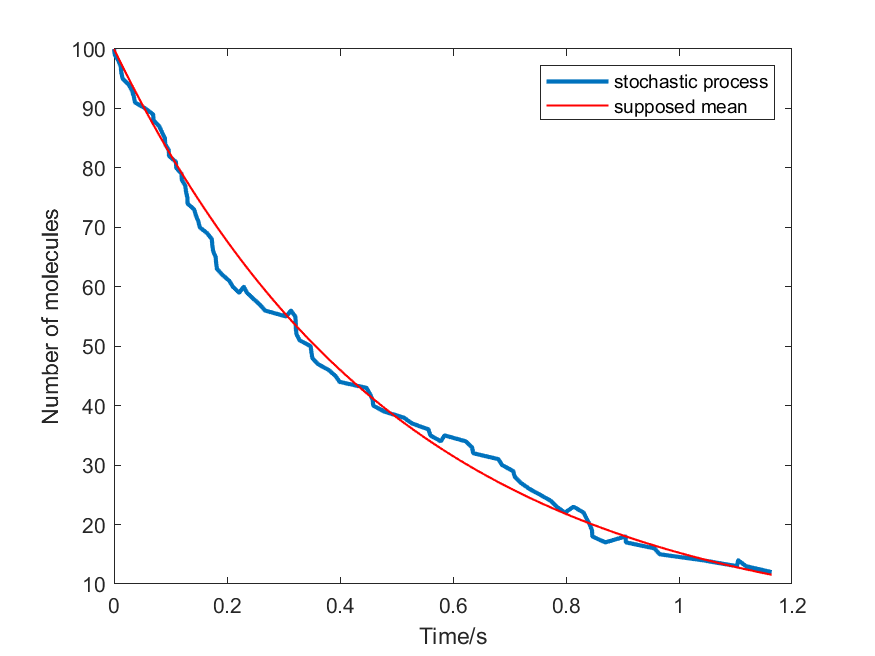
\includegraphics[width=\linewidth]{graph/c2.png}
        \caption{Simulation2}
        \label{c2}
    \end{minipage}
\end{figure}
\begin{figure}[htbp]
    \centering
    \begin{minipage}{0.45\linewidth}
        \centering
        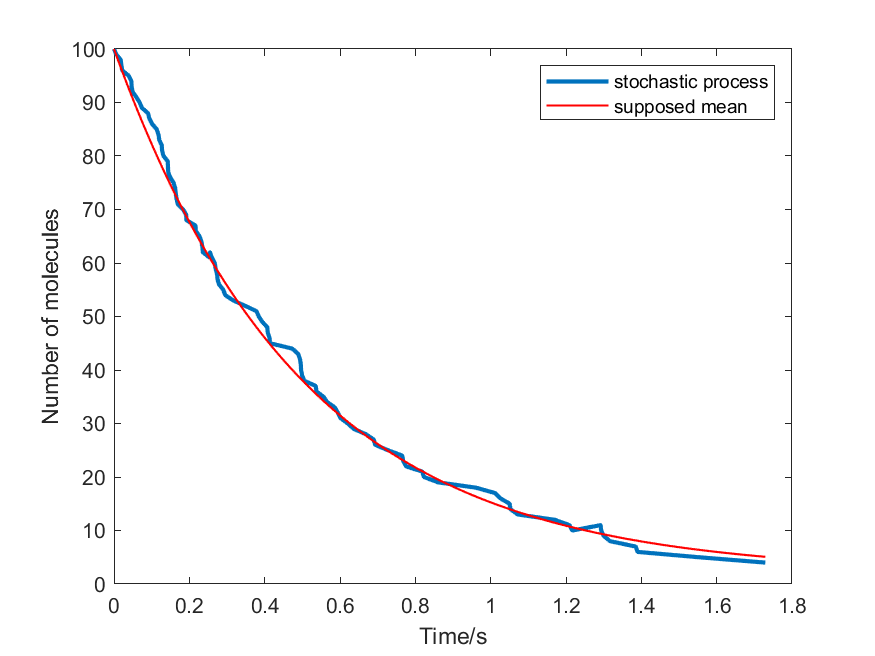
\includegraphics[width=\linewidth]{graph/c3.png}
        \caption{Simulation3}
        \label{c3}
    \end{minipage}
    \hfill
    \begin{minipage}{0.45\linewidth}
        \centering
        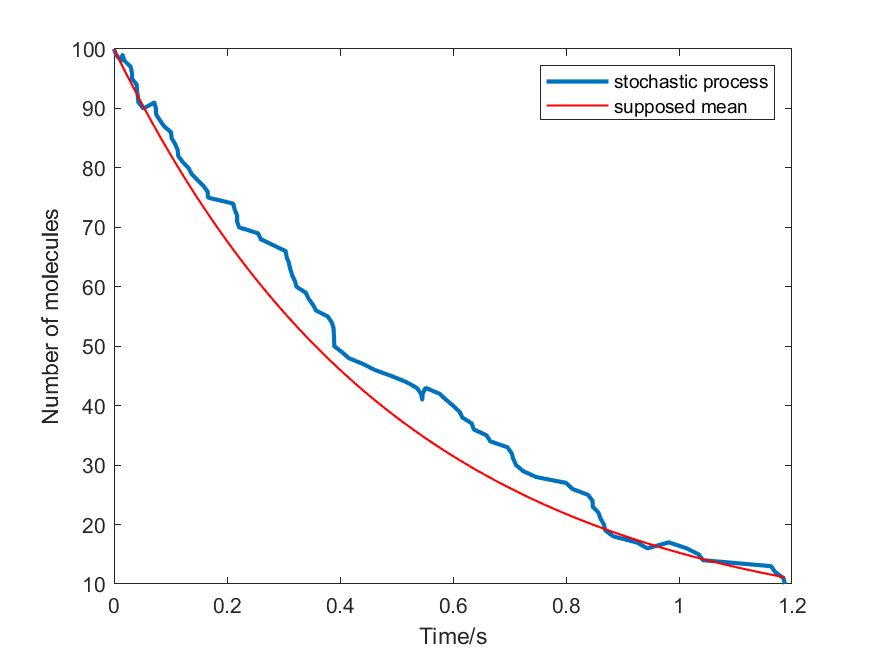
\includegraphics[width=\linewidth]{graph/c4.png}
        \caption{Simulation4}
        \label{c4}
    \end{minipage}
\end{figure}
\begin{figure}[htbp]
    \centering
    \begin{minipage}{0.45\linewidth}
        \centering
        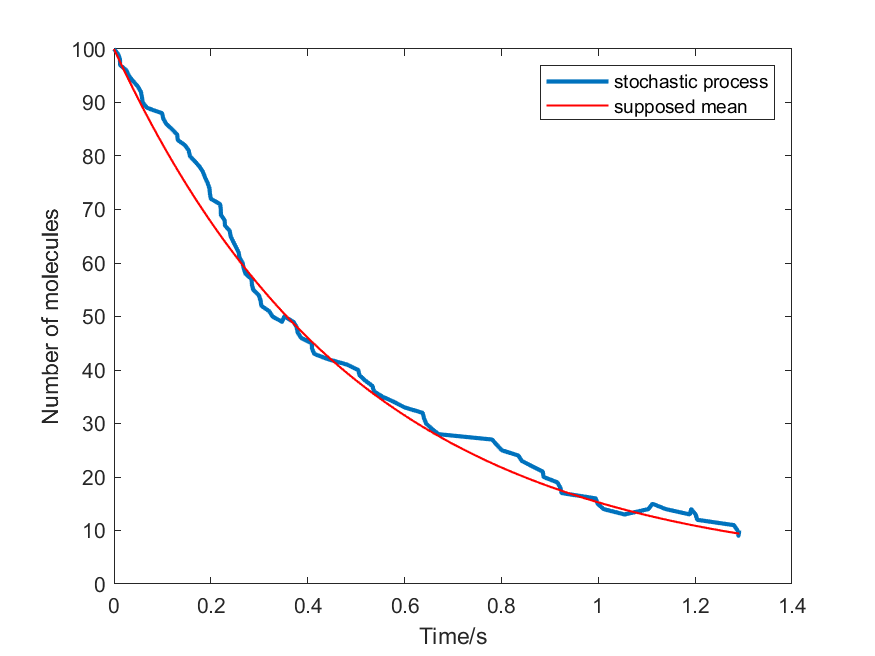
\includegraphics[width=\linewidth]{graph/c5.png}
        \caption{Simulation5}
        \label{c5}
    \end{minipage}
    \hfill
    \begin{minipage}{0.45\linewidth}
        \centering
        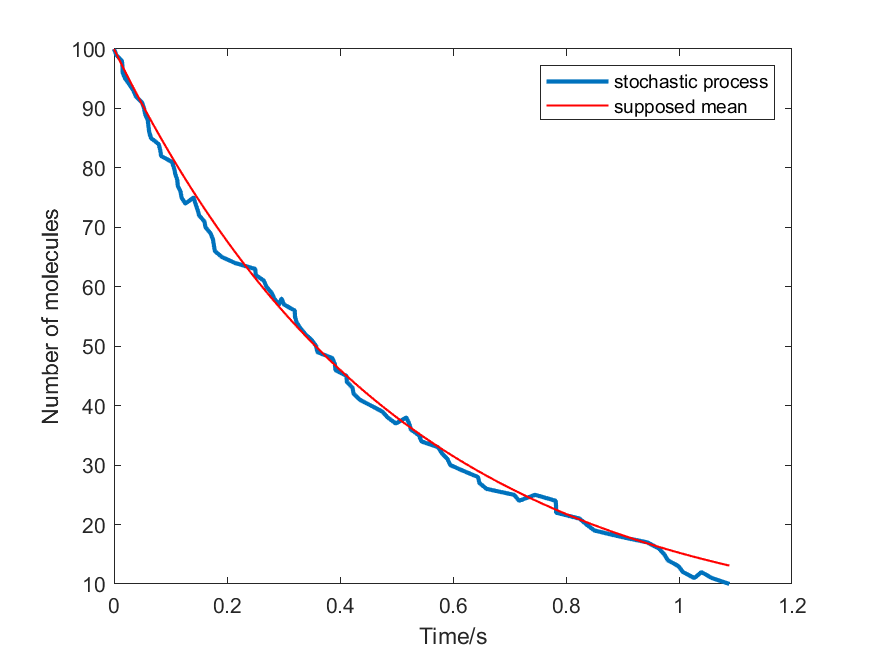
\includegraphics[width=\linewidth]{graph/c6.png}
        \caption{Simulation6}
        \label{c6}
    \end{minipage}
\end{figure}
\begin{figure}[htbp]
    \centering
    \begin{minipage}{0.45\linewidth}
        \centering
        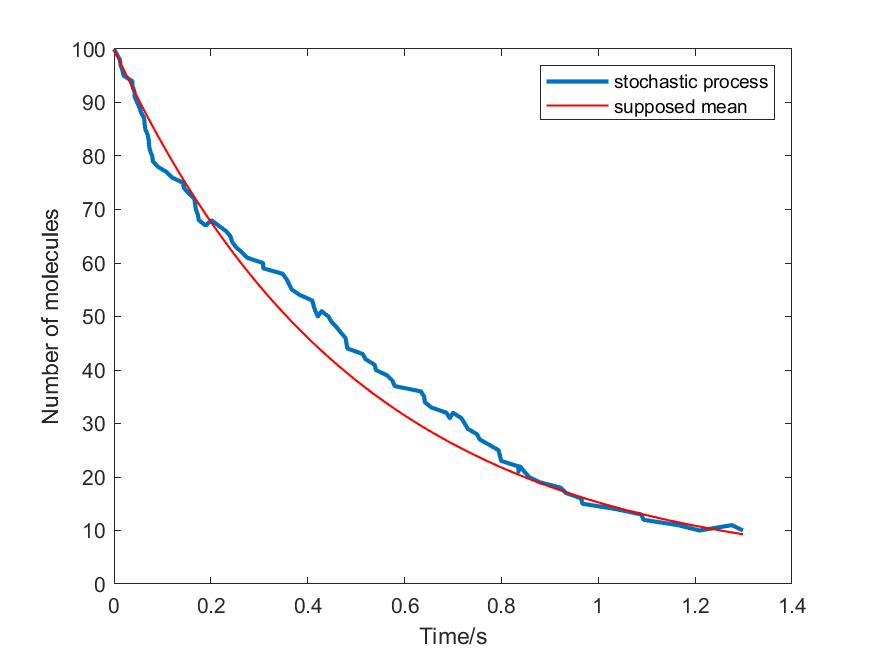
\includegraphics[width=\linewidth]{graph/c7.png}
        \caption{Simulation7}
        \label{c7}
    \end{minipage}
    \hfill
    \begin{minipage}{0.45\linewidth}
        \centering
        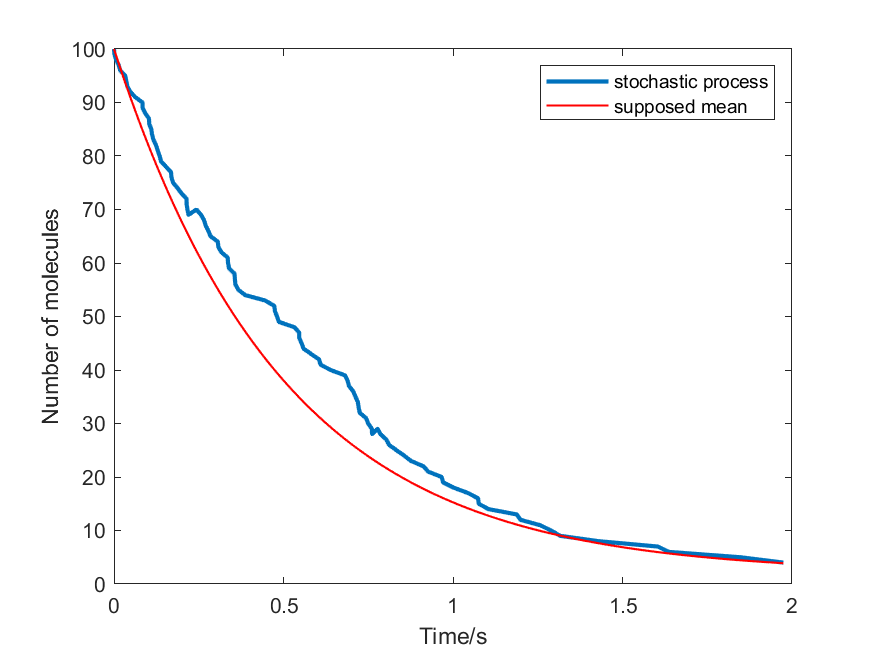
\includegraphics[width=\linewidth]{graph/c8.png}
        \caption{Simulation8}
        \label{c8}
    \end{minipage}
\end{figure}
\begin{figure}[htbp]
    \centering
    \begin{minipage}{0.45\linewidth}
        \centering
        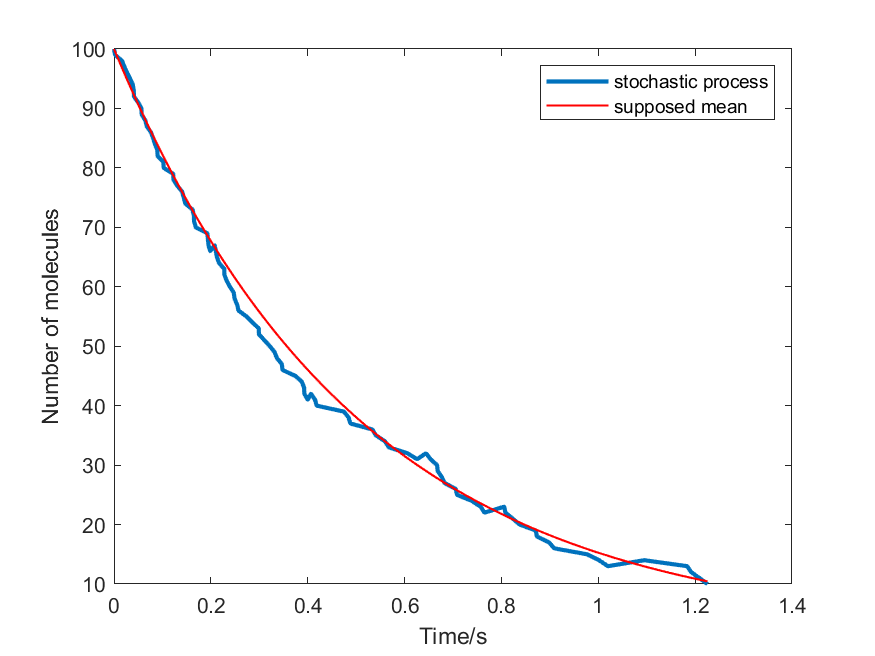
\includegraphics[width=\linewidth]{graph/c9.png}
        \caption{Simulation9}
        \label{c9}
    \end{minipage}
    \hfill
    \begin{minipage}{0.45\linewidth}
        \centering
        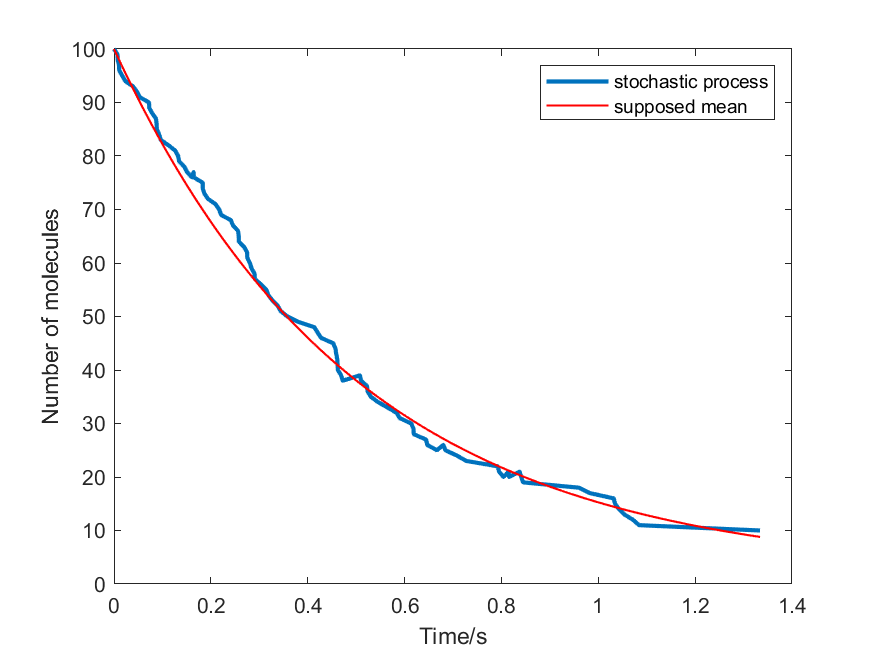
\includegraphics[width=\linewidth]{graph/c10.png}
        \caption{Simulation10}
        \label{c10}
    \end{minipage}
\end{figure}
\begin{figure}[htbp]
\centering
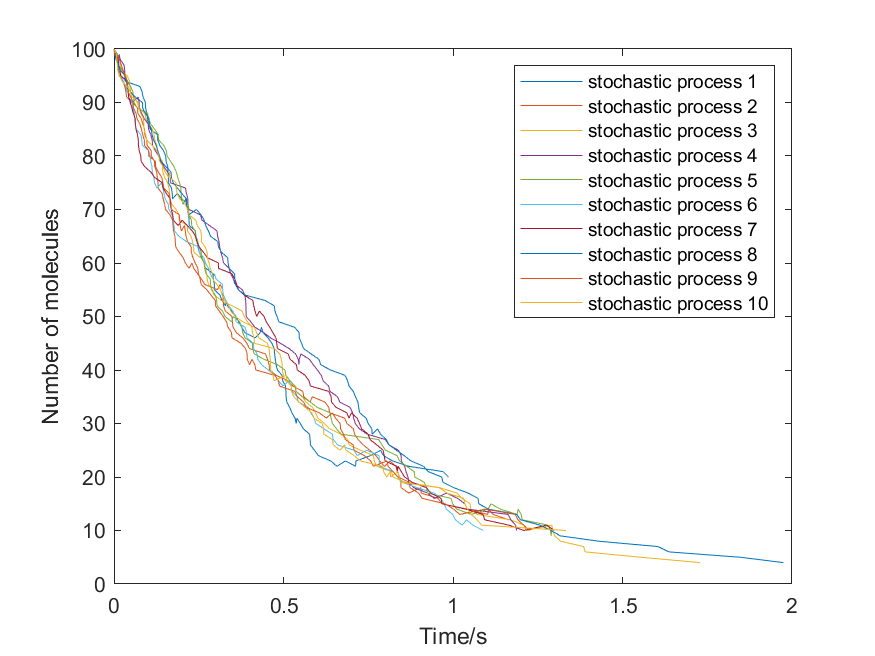
\includegraphics[width=\linewidth]{graph/mean2.png}
\caption{mean}
\end{figure}
\clearpage









\section{code}
\subsection{"Naive" stochastic simulation}
\begin{lstlisting}
k=2;
deltat=0.001;
n0=1000;
naivess1(k,deltat,n0);
function naivess1(k,deltat,n0)
A=n0;
a=n0;
while a>0
    r=rand;
    if r<a*k*deltat
        a=a-1;
    end
    A=vertcat(A,a);
end
[m,n]=size(A);
x=linspace(deltat,m*deltat,m);
plot(x,A);
end
\end{lstlisting}

\subsection{Gillespie stochastic simulation algorithm}
\begin{lstlisting}
k=2;
deltat=0.01;
n0=100;
T1=gillespie(k,deltat,n0,'b1.png');
T2=gillespie(k,deltat,n0,'b2.png');
T3=gillespie(k,deltat,n0,'b3.png');
T4=gillespie(k,deltat,n0,'b4.png');
T5=gillespie(k,deltat,n0,'b5.png');
T6=gillespie(k,deltat,n0,'b6.png');
T7=gillespie(k,deltat,n0,'b7.png');
T8=gillespie(k,deltat,n0,'b8.png');
T9=gillespie(k,deltat,n0,'b9.png');
T10=gillespie(k,deltat,n0,'b10.png');
x=linspace(n0,0,n0+1);
plot(T1,x,'DisplayName','stochastic process 1');hold on
plot(T2,x,'DisplayName','stochastic process 2');
plot(T3,x,'DisplayName','stochastic process 3');
plot(T4,x,'DisplayName','stochastic process 4');
plot(T5,x,'DisplayName','stochastic process 5');
plot(T6,x,'DisplayName','stochastic process 6');
plot(T7,x,'DisplayName','stochastic process 7');
plot(T8,x,'DisplayName','stochastic process 8');
plot(T9,x,'DisplayName','stochastic process 9');
plot(T10,x,'DisplayName','stochastic process 10');
legend()
ylabel('Number of molecules')
xlabel('Time/s')
hold off
saveas(gcf, 'mean1.png');
function T=gillespie(k,deltat,n0,name)
T=linspace(0,n0,n0+1);
t=0;
a=n0;
for i=2:n0+1
    r=rand;
    t=t+log(1/r)/(a*k);
    a=a-1;
    T(i)=t;
end
x=linspace(n0,0,n0+1);
plot(T,x, 'LineWidth', 2,'DisplayName', 'stochastic process');hold on
T2=linspace(0,T(n0+1),1000);
Y=n0*exp(-k*T2);
plot(T2,Y,'r', 'LineWidth', 1,'DisplayName', 'supposed mean');
hold off
legend()
ylabel('Number of molecules')
xlabel('Time/s')
saveas(gcf, name);
end
\end{lstlisting}

\subsection{Gillespie SSA for 2 reactions}
\begin{lstlisting}
k1=2;
k2=4;
n0=100;
[T1,A1]=gillespie2(k1,k2,n0,'c1.png');
[T2,A2]=gillespie2(k1,k2,n0,'c2.png');
[T3,A3]=gillespie2(k1,k2,n0,'c3.png');
[T4,A4]=gillespie2(k1,k2,n0,'c4.png');
[T5,A5]=gillespie2(k1,k2,n0,'c5.png');
[T6,A6]=gillespie2(k1,k2,n0,'c6.png');
[T7,A7]=gillespie2(k1,k2,n0,'c7.png');
[T8,A8]=gillespie2(k1,k2,n0,'c8.png');
[T9,A9]=gillespie2(k1,k2,n0,'c9.png');
[T10,A10]=gillespie2(k1,k2,n0,'c10.png');
plot(T1,A1,'DisplayName','stochastic process 1');hold on
plot(T2,A2,'DisplayName','stochastic process 2');
plot(T3,A3,'DisplayName','stochastic process 3');
plot(T4,A4,'DisplayName','stochastic process 4');
plot(T5,A5,'DisplayName','stochastic process 5');
plot(T6,A6,'DisplayName','stochastic process 6');
plot(T7,A7,'DisplayName','stochastic process 7');
plot(T8,A8,'DisplayName','stochastic process 8');
plot(T9,A9,'DisplayName','stochastic process 9');
plot(T10,A10,'DisplayName','stochastic process 10');
legend()
ylabel('Number of molecules')
xlabel('Time/s')
hold off
saveas(gcf, 'mean2.png');
function [T,A]=gillespie2(k1,k2,n0,name)
T=linspace(0,100,101);
A=linspace(0,101,101);
t=0;
A(1)=n0;
a=n0;
for i=2:101
    r1=rand;
    r2=rand;
    alpha=a*k1+k2;
    t=t+log(1/r1)/(alpha);
    if r2<k2/alpha
        a=a+1;
    else
        a=a-1;
    end
    A(i)=a;
    T(i)=t;
end
plot(T,A, 'LineWidth', 2,'DisplayName', 'stochastic process');hold on
T2=linspace(0,T(101),1000);
Y=k2/k1+(n0-k2/k1)*exp(-k1*T2);
plot(T2,Y,'r', 'LineWidth', 1,'DisplayName', 'supposed mean');
hold off
legend()
ylabel('Number of molecules')
xlabel('Time/s')
saveas(gcf,name);
end
\end{lstlisting}



\end{document}